\chapter{Wyniki}

\indent\indent Przeprowadzono uruchomienie programu dla dwóch profili lotniczych: symetrycznego \textsf{NACA 0012} oraz \textsf{NACA 8207}. Współrzędne punktów tworzących ich obrysy zaczerpnięto ze strony internetowej \url{http://www.ae.illinois.edu/m-selig/ads/coord_database.html}. Ze względu na użycie w projekcie naiwnego sposobu generowania siatki obliczeniowej, o jednorodnym odstępie między węzłami w kierunku $v$, zdecydowano się na zagęszczenie siatki do stu rzędów. Do celów porównawczych dla każdego z przypadków przeprowadzono obliczenia metodą siłową. Otrzymane pliki wyjściowe \textsf{.dat} wczytano do programu \textsf{Tecplot}, a wygenerowane mapy konturowe przedstawiono poniżej na rysunkach. Na końcu rozdziału zaprezentowano wykresy obliczonej odległości dla pierwszego rzędu siatki.

%Rysunki całego obszaru obliczeniowego NACA 0012
\begin{figure}[h]	
    \begin{subfigure}[h]{\textwidth}
    	\centering
    	\includegraphics[trim = 22mm 10mm 10mm 20mm, width=0.9\linewidth]{Rysunki/NACA_0012_profil_brute.eps}
    	\subcaption{Metoda siłowa}	    	
	\end{subfigure}    
	\begin{subfigure}[h]{\textwidth}
		\centering
    	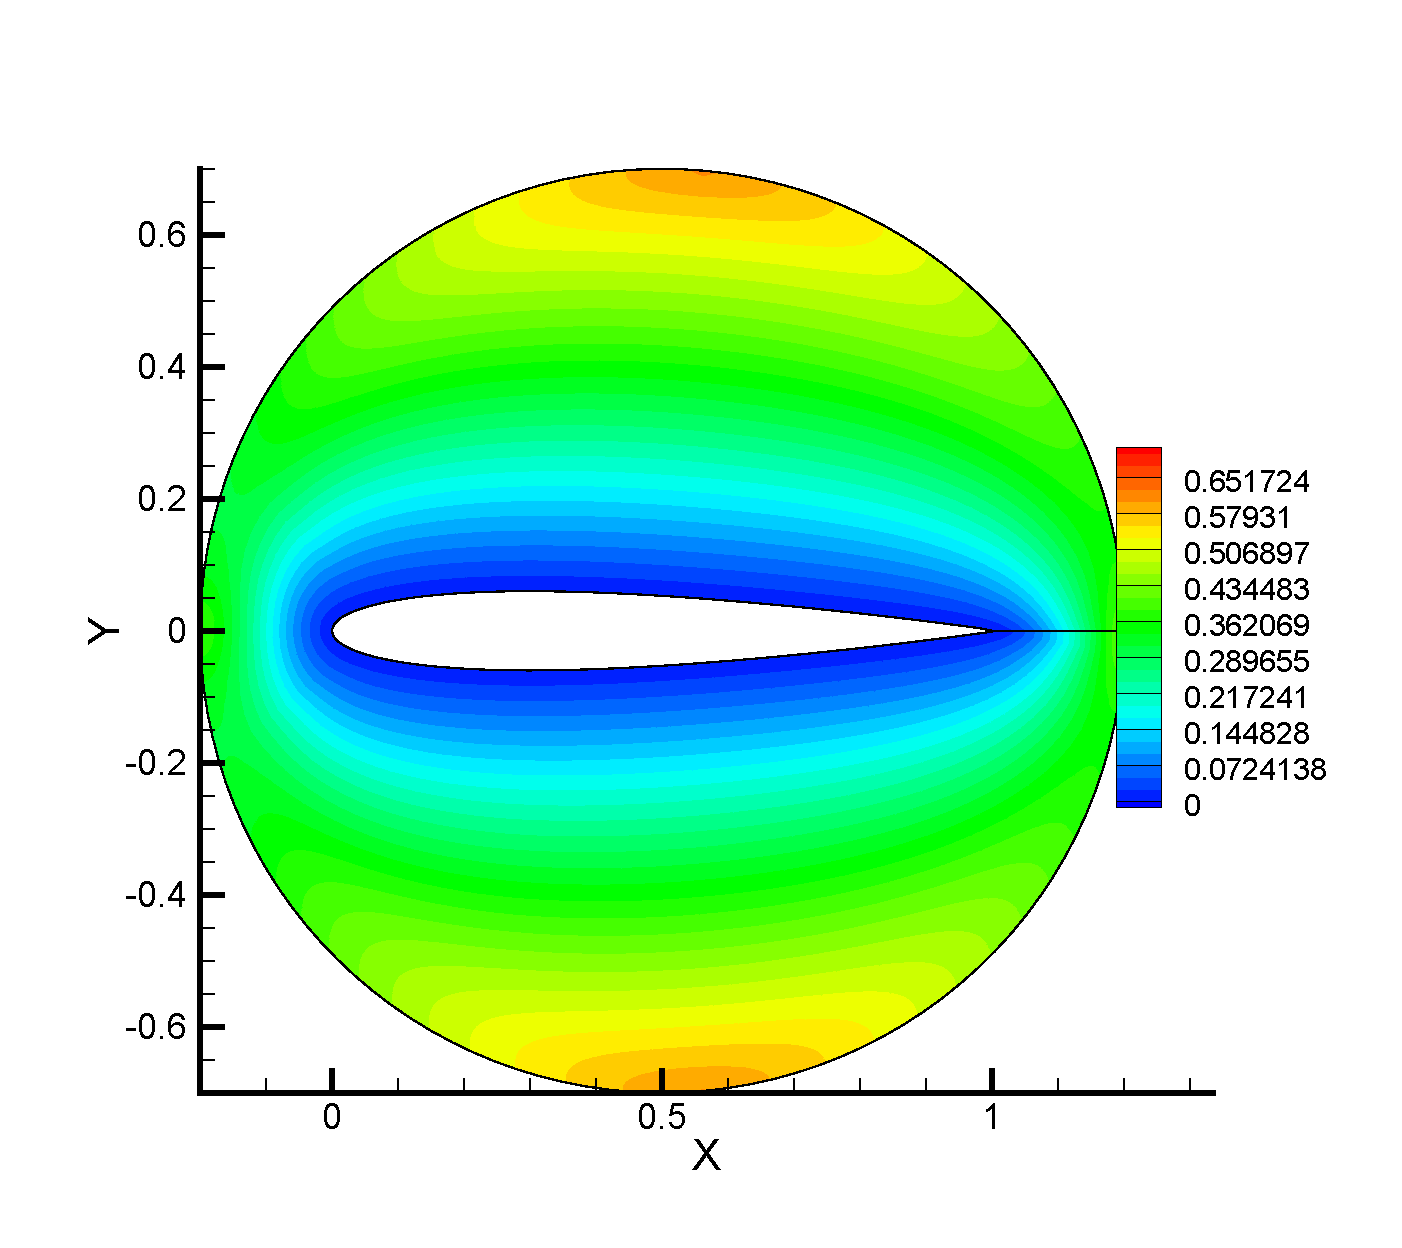
\includegraphics[trim = 22mm 10mm 10mm 20mm, width=0.9\linewidth]{Rysunki/NACA_0012_profil_poisson.eps}      	
    	\subcaption{Metoda Poissona}
	\end{subfigure}
	\caption{Profil NACA 0012}
\end{figure}

\begin{figure}[h]	
    \begin{subfigure}[h]{\textwidth}
    	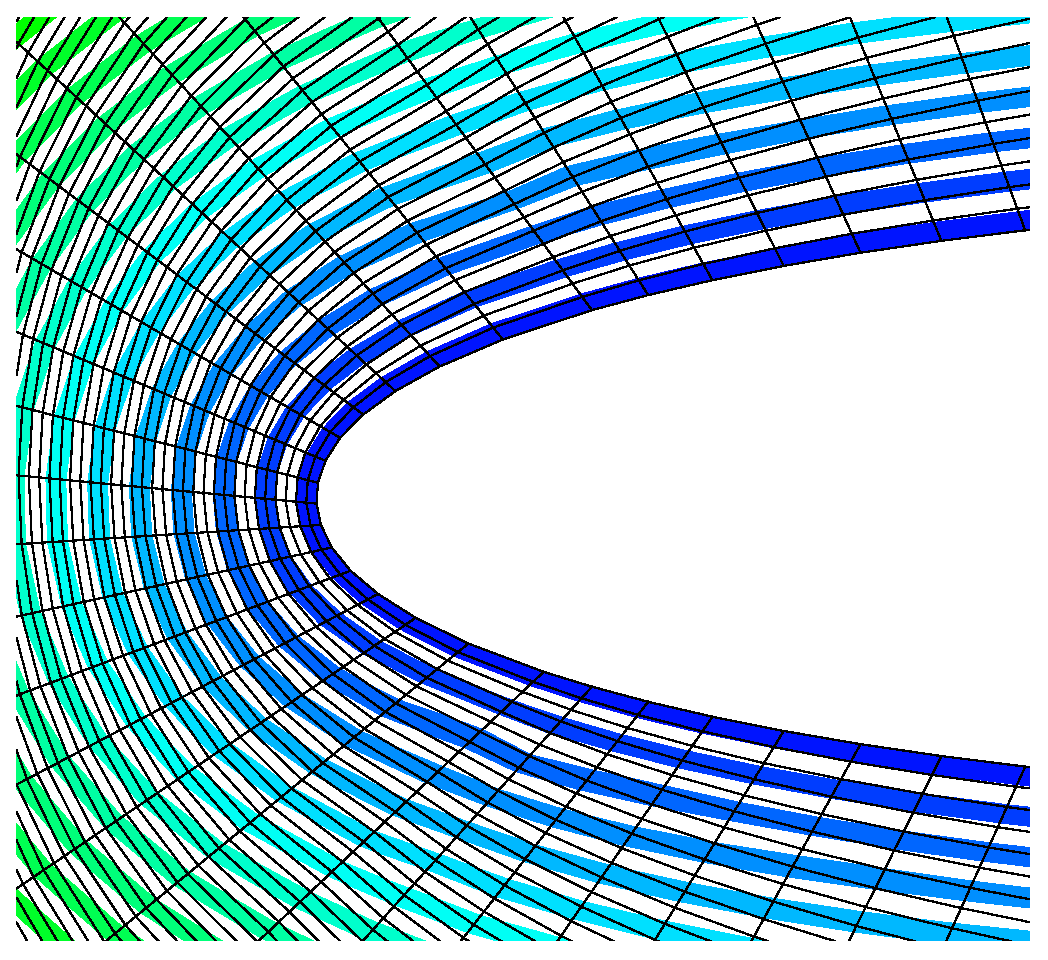
\includegraphics[width=0.5\textwidth]{Rysunki/NACA_0012_nosek_brute}  
    	\quad      
    	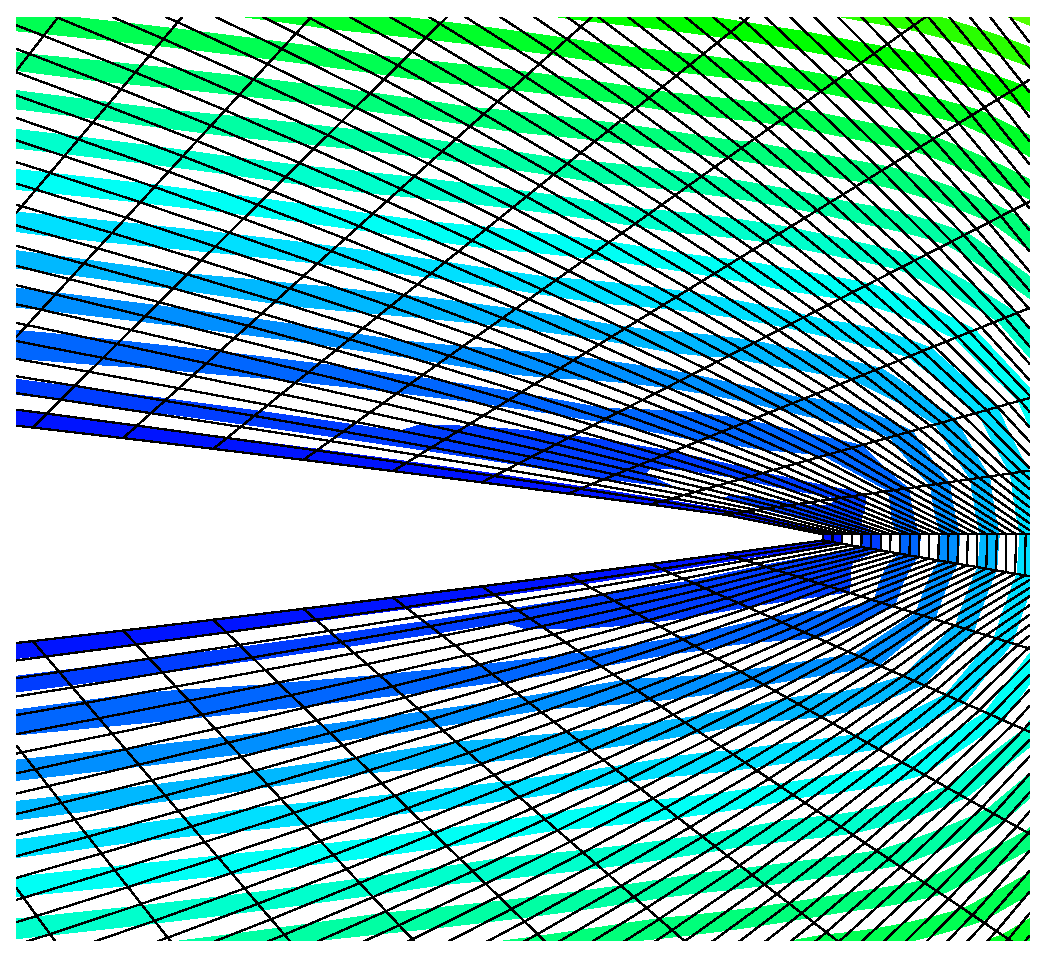
\includegraphics[width=0.5\textwidth]{Rysunki/NACA_0012_ostrze_brute}
    	\subcaption{Metoda siłowa}
    	\vspace{1cm}
	\end{subfigure}
	    
	\begin{subfigure}[h]{\textwidth}
    	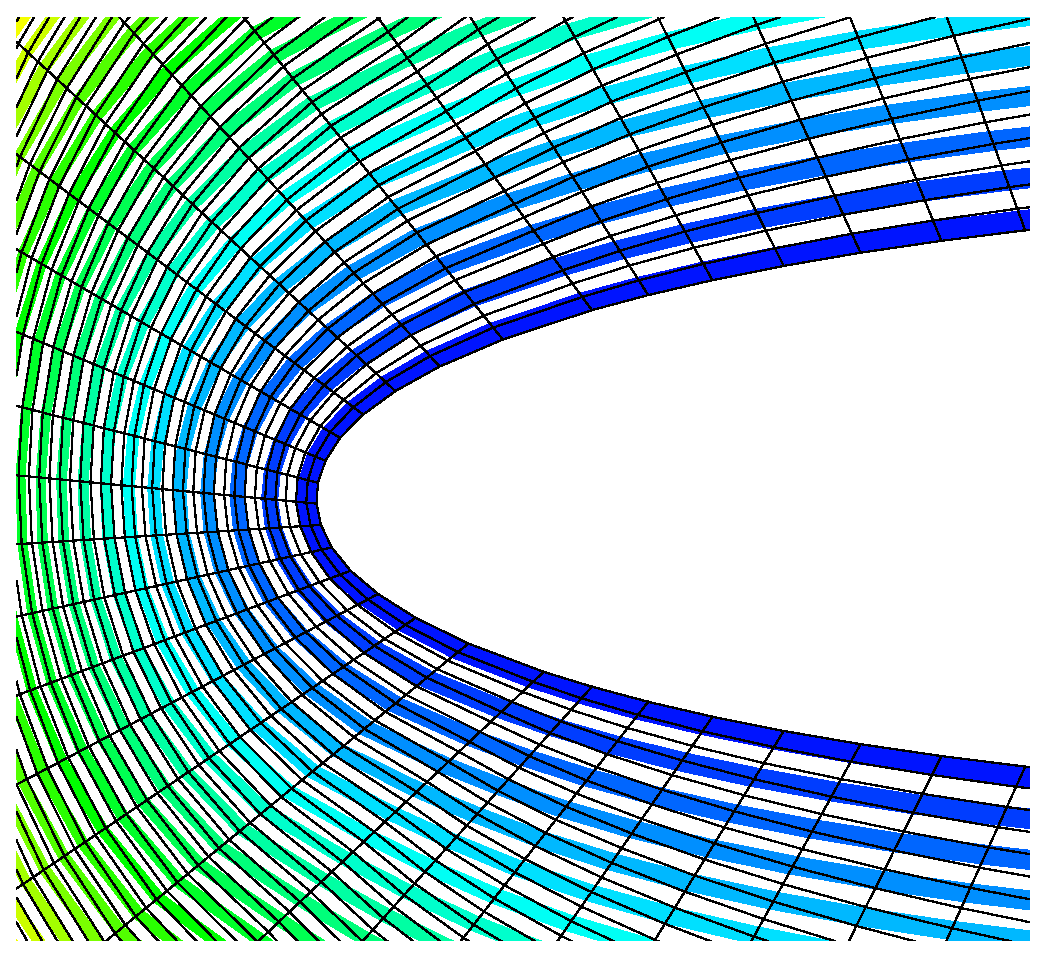
\includegraphics[width=0.5\textwidth]{Rysunki/NACA_0012_nosek_poisson}  
    	\quad      
    	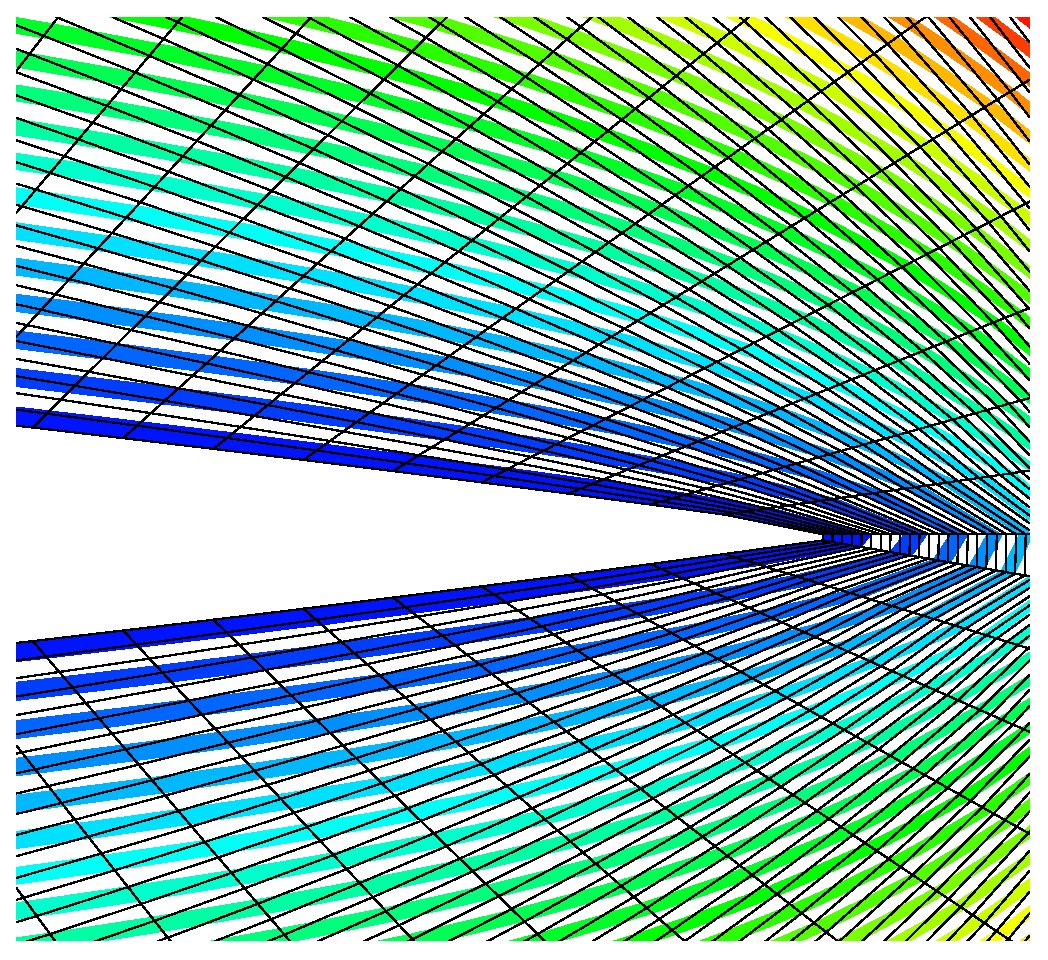
\includegraphics[width=0.5\textwidth]{Rysunki/NACA_0012_ostrze_poisson}		
		\subcaption{Metoda Poissona}
	\end{subfigure}
	\caption{Profil NACA 0012 (po lewej nosek profilu, po prawej ostrze)}
\end{figure}

%Rysunki całego obszaru obliczeniowego NACA 8207
\begin{figure}[h]	
    \begin{subfigure}[h]{\textwidth}
    	\centering
    	\includegraphics[trim = 22mm 10mm 10mm 20mm, width=0.9\linewidth]{Rysunki/NACA_8207_profil_brute}
    	\subcaption{Metoda siłowa}	    	
	\end{subfigure}    
	\begin{subfigure}[h]{\textwidth}
		\centering
    	\includegraphics[trim = 22mm 10mm 10mm 20mm, width=0.9\linewidth]{Rysunki/NACA_8207_profil_poisson}      	
    	\subcaption{Metoda Poissona}
	\end{subfigure}
	\caption{Profil NACA 8207}
\end{figure}

\begin{figure}[h]	
    \begin{subfigure}[h]{\textwidth}
    	%\centering
    	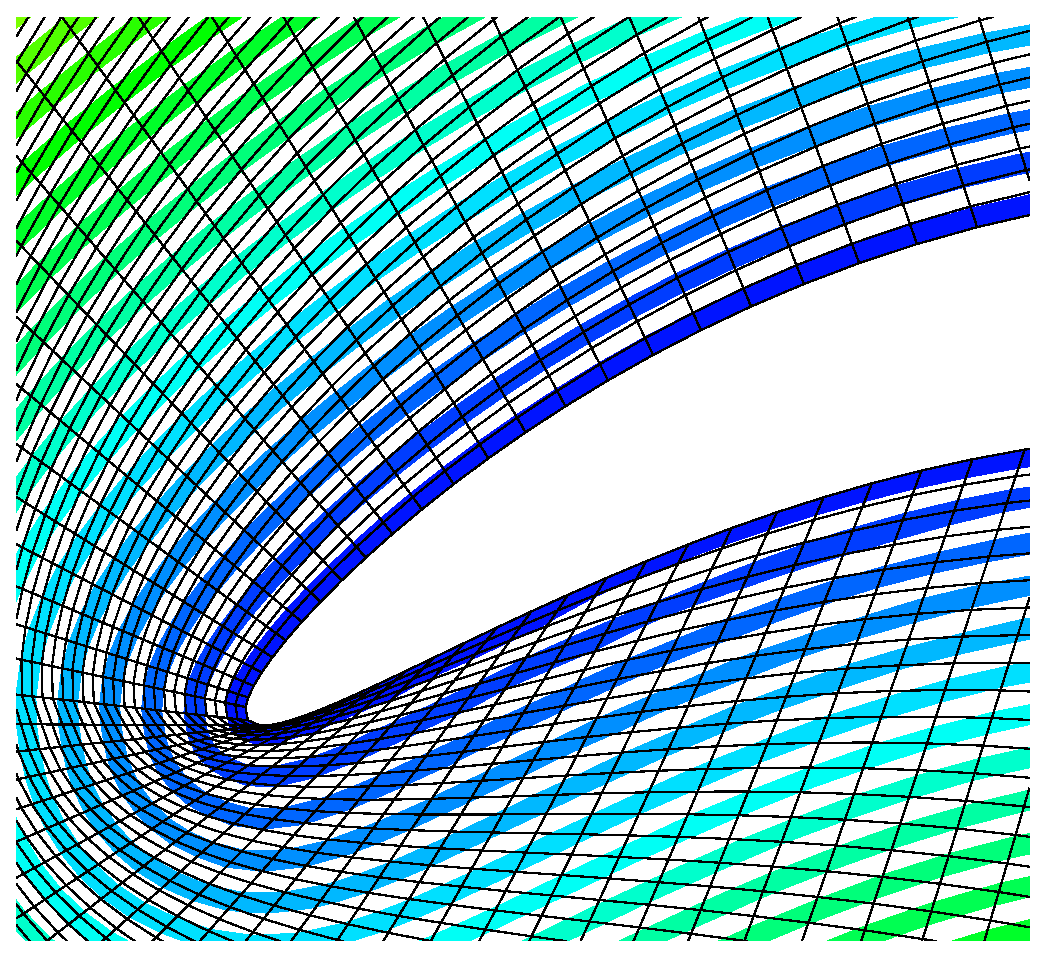
\includegraphics[width=0.5\textwidth]{Rysunki/NACA_8207_nosek_brute}  
    	\quad      
    	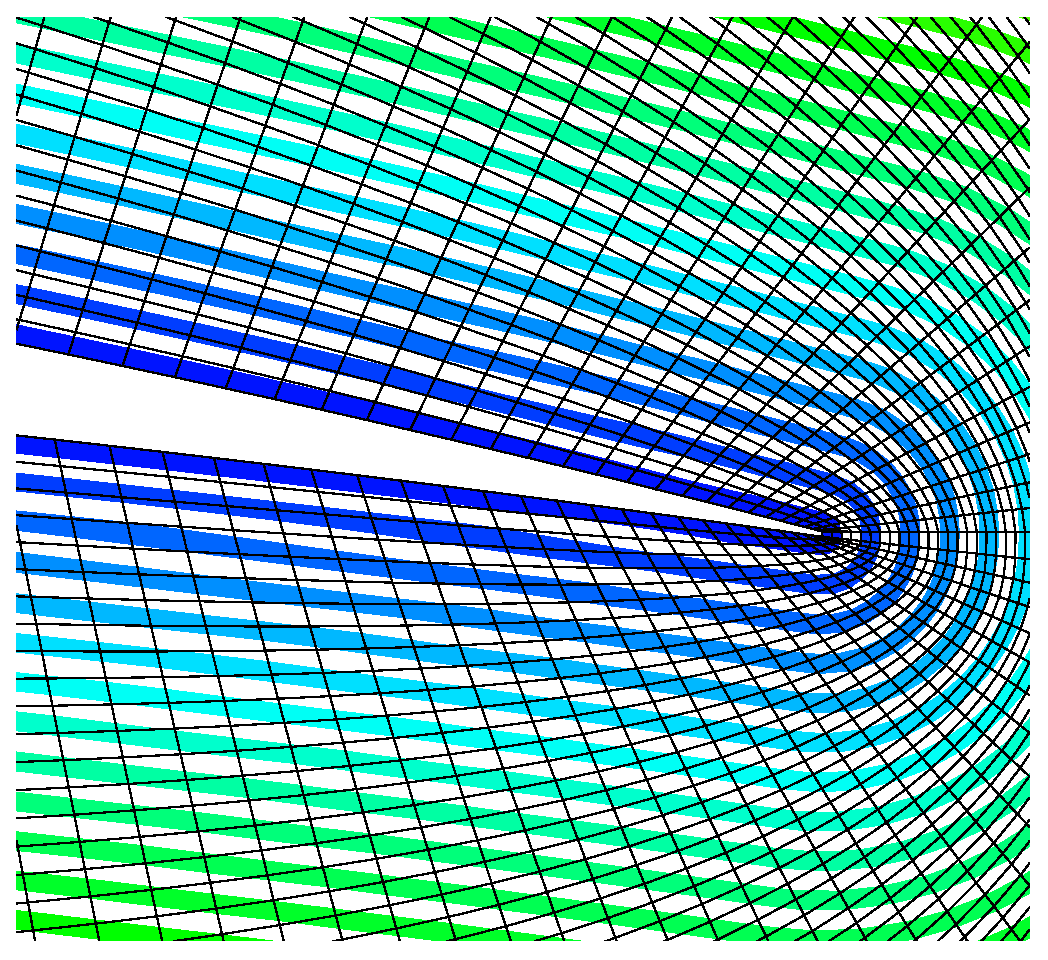
\includegraphics[width=0.5\textwidth]{Rysunki/NACA_8207_ostrze_brute}
    	\subcaption{Metoda siłowa}
    	\vspace{1cm}
	\end{subfigure}
    
	\begin{subfigure}[h]{\textwidth}
    	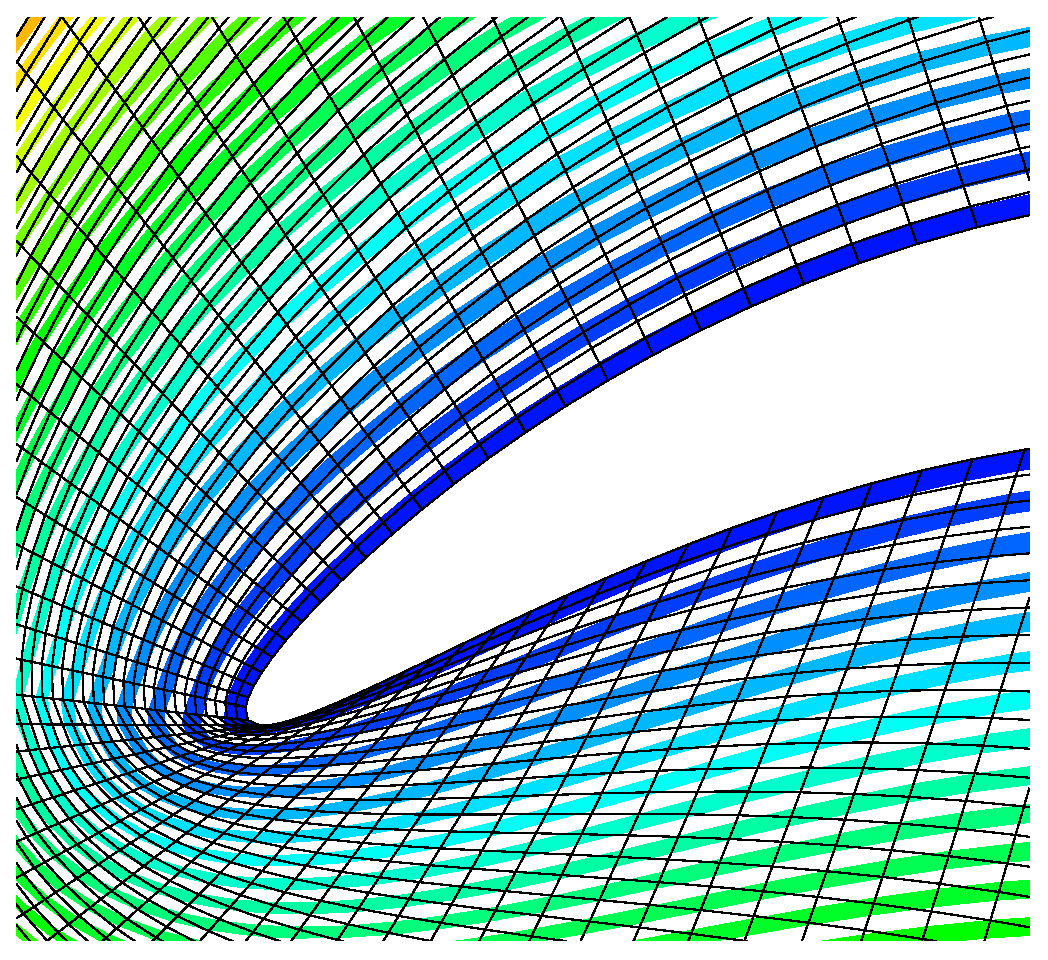
\includegraphics[width=0.5\textwidth]{Rysunki/NACA_8207_nosek_poisson}  
    	\quad      
    	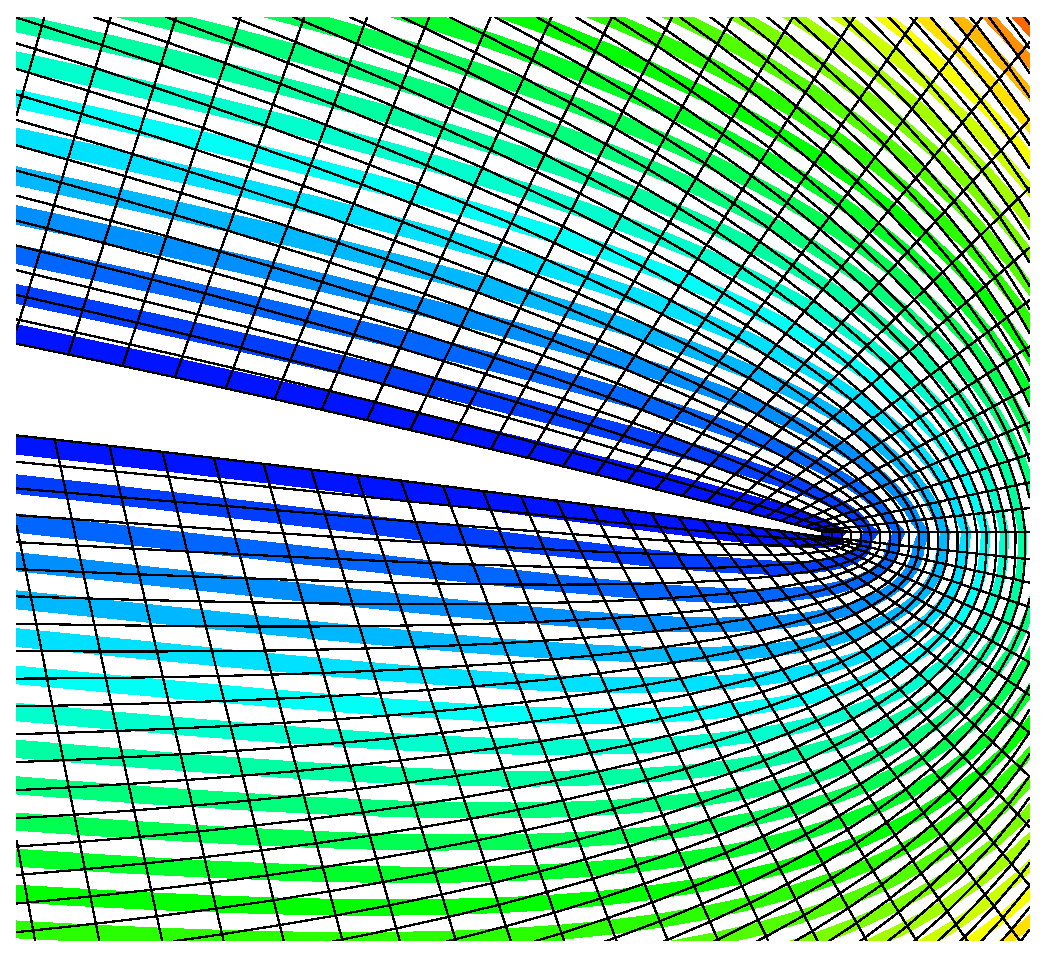
\includegraphics[width=0.5\textwidth]{Rysunki/NACA_8207_ostrze_poisson}		
		\subcaption{Metoda Poissona}
	\end{subfigure}
	\caption{Profil NACA 8207 (po lewej nosek profilu, po prawej ostrze)}
\end{figure}

\begin{figure}[b] 
	\includegraphics[trim = 30mm 0mm 0mm 0mm, width=1.1\linewidth]{Rysunki/NACA_0012_wykres_odleglosci.png}
	\caption{Wykres odległości dla pierwszego rzędu siatki dla metody \colorbox{red!30}{Poissona} i \colorbox{blue!30}{siłowej} (NACA 0012). Kolorem zielonym oznaczono \colorbox{green!30}{błąd bezwzględny}.}
	\label{fig:graph_NACA_0012}
\end{figure}

\begin{figure}[b] 
	\includegraphics[trim = 30mm 0mm 0mm 0mm, width=1.1\linewidth]{Rysunki/NACA_8207_wykres_odleglosci.png}
	\caption{Wykres odległości dla pierwszego rzędu siatki dla metody \colorbox{blue!30}{Poissona} i \colorbox{red!30}{siłowej} (NACA 8207). Kolorem zielonym oznaczono \colorbox{green!30}{błąd bezwzględny}.}
	\label{fig:graph_NACA_8207}
\end{figure}